\FILE{design}

\section{Design}

To fulfill our requirements we have developed a framework for workflow
controlled computing called Cloudmesh compute cluster that we call
{\em Cloudmesh-cc}. The architecture of the framework is depicted in
Figure~\ref{fig:arch}.

\begin{figure}[htb]
\centering
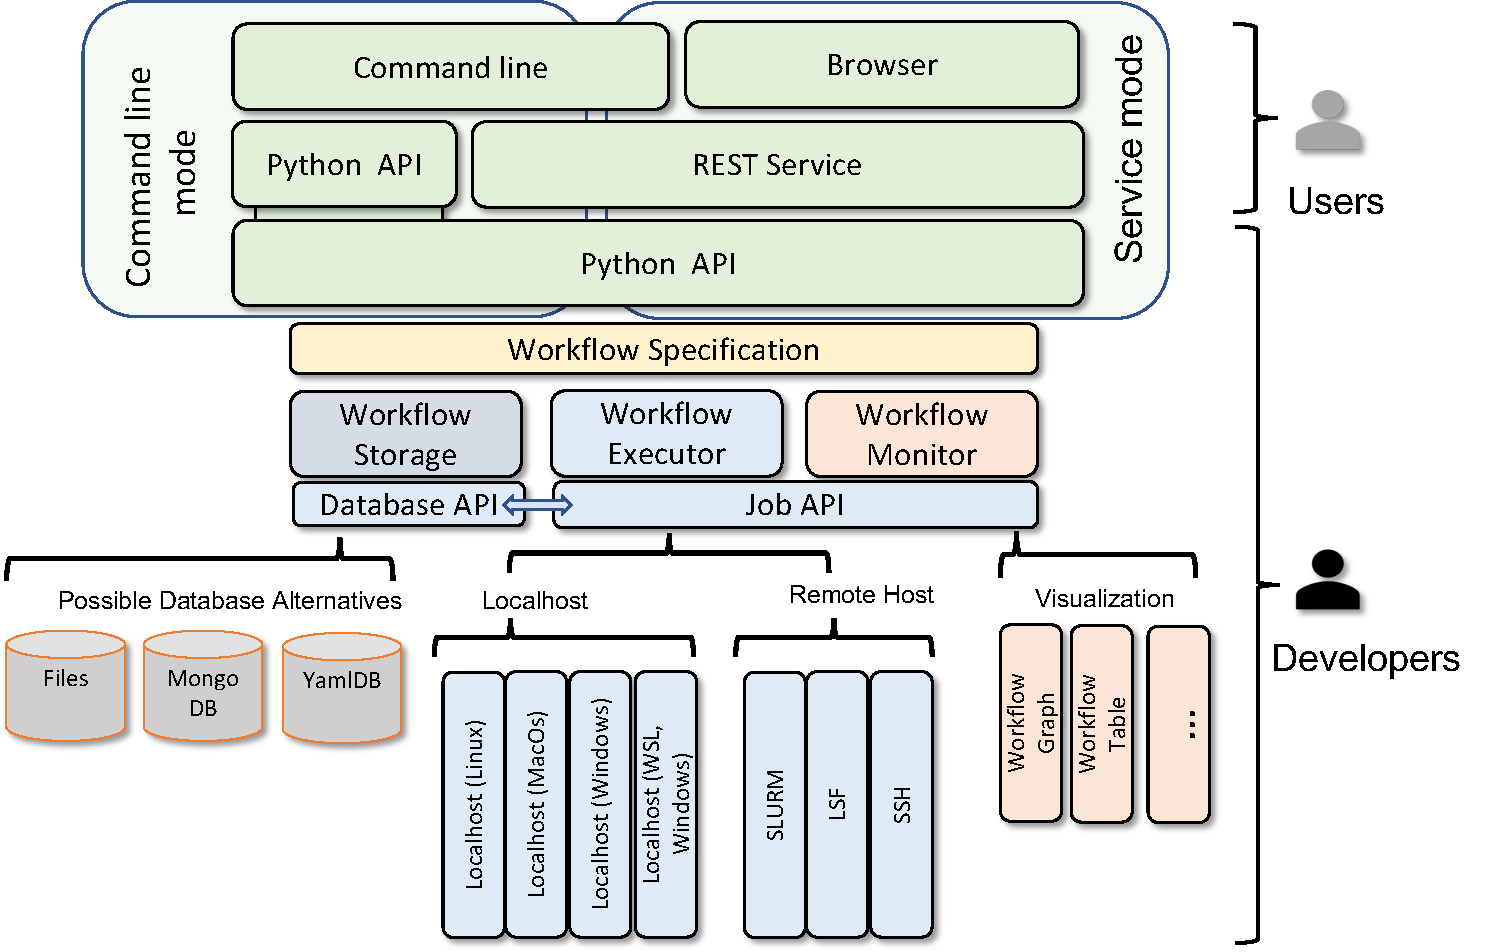
\includegraphics[width=1.0\columnwidth]{images/cloudmesh-cc-arch.pdf}
\caption{Architecture of the Cloudmesh-cc Framework}\label{fig:arch}
\end{figure}

The framework is based on a layered architecture so it can be improved
and expanded on at each layer. We distinguish two kinds of users,
developers and endusers that define their own workflows to run on
compute resources. For the end user we provide a commandline and a
very simple browser interface. The simplicity is important as it does
not require to spend exorbitant amounts of time to learn how to use
the workflow framework. To support developers we have designed a
minimal Python API that is also used to implement a REST Service.
Currently the REST service is supposed to run on the client, but a
service deployment could also be conducted while assuring that proper
authentication and authorization is used. This is easily possible as
we use a well-known REST service framework (FastAPI) that can integrate
with common security frameworks to secure services. The API, workflow
specification, commandline interface, and browser are well documented
with the help of Sphinx and OpenAPI.

The workflow specification plays an important role to not only define
a workflow, but also to keep the status of a currently executed
workflow. Here we have completely separated the status of the workflow
and synchronize the state of the Workflow with pull requests to the
service that executes the computation. This allows the system to be
shut down at any time while the running jobs are completely
independent from the client application accessing the state. Thus the
client appears to be stateless and fetches the state of the submitted
jobs on demand. It will return the latest state found on the job
execution services.

The workflows are defined with YAML. The workflow is stored in a
database that can be implemented using a variety of backends such as
YamlDB which is file based, MongoDB, or pickle. In our current
implementation we just use a file-based implementation as it does not
require to set up and manage more complex databases. This is an
important capability as we found that scientists and beginning
students do not want to engage in the hassle of setting up and
managing a datastore such as MongoDB.

As we use a YAML file to represent the status of the workflow it is
easy to create monitoring components for example as part of a Web
browser. Various graph sophisticated display frameworks could be
used. For now we have simply exposed the graph in table format using
datatables.net and the graph as SVG while leveraging Graphviz.

One of the most important parts of the framework is how we manage jobs
and monitor their status. For this, we have introduced a abstract job
class that is integrated in our workflow class. The job class has the
ability to define jobs, start them, and cancel them, to name only the
most important management methods. However, each job defines a status
file in which the actual progress of the job is recorded. This status
file is managed on the compute resource where the job is run and is
queried on demand to return the status to the client. This way, the
status of all jobs can be monitored. As our goal is not to run jobs
that execute in milliseconds, but rather than in the second range such
status reporting and propagation is well suited for us. We have
defined a special status progress update specification that is
universally applicable. These jobs can be bash scripts, Python scripts,
Jupyter notebooks, or Slurm scripts.

Workflows are compilations of jobs to be run on nodes. These workflows
report information on the status of jobs as they are run, whether
locally or remotely.  These types of jobs can be mixed
with one another in a single workflow. This allows us, as already mentioned, 
to view the progress of a workflow as it is being run in quasi-realtime.
The workflow can be monitored as a graph or a datatable. These interfaces
report the statuses of the jobs. Additionally, the order in which the jobs
are run can be specified, enabling prerequisite jobs and the segmentation of a
workflow.

To address the requirement of simplicity the overall code is less than
3600 lines of code with additional 2600 lines for extensive test
cases.

The framework is managed as OpenSource repository in GitHub and uses
Python as the implementation language. The code is compatible with
Windows, macOS, and Linux.
